\documentclass[10pt,a4paper,twocolumn]{article}
%\documentclass[12pt,a4paper]{article}


\usepackage[T2A]{fontenc}
\usepackage[utf8]{inputenc}

\usepackage{amsmath}
\usepackage{commath}
\usepackage{titlesec}
\usepackage{caption}
\usepackage{indentfirst}
\usepackage{hyperref}
\usepackage{enumitem}[leftmargin=0pt]
\usepackage{multicol}
\usepackage{yfonts}
\usepackage{verbatim}
\usepackage{bm}
\usepackage{float}

\usepackage[backend=biber]{biblatex}
\addbibresource{ref.bib}

\usepackage{graphicx}
\graphicspath{{./images/}}

\renewcommand{\vec}[1]{\bm{\mathrm{#1}}}


\begin{document}

\title{Resonance Curve of a Physical Pendulum}
\author{Aleksandar Ivanov}
\date{\today}
\maketitle

\section{Problem statement}

We excite a physical pendulum with a sinusoidal driving torque in such a way that it achieves a significant amplitude. Describe the shape of the nonlinear resonance curve.

\section{Mathematical setup}

\begin{figure}[h]
\centering
\captionsetup{justification=centering}
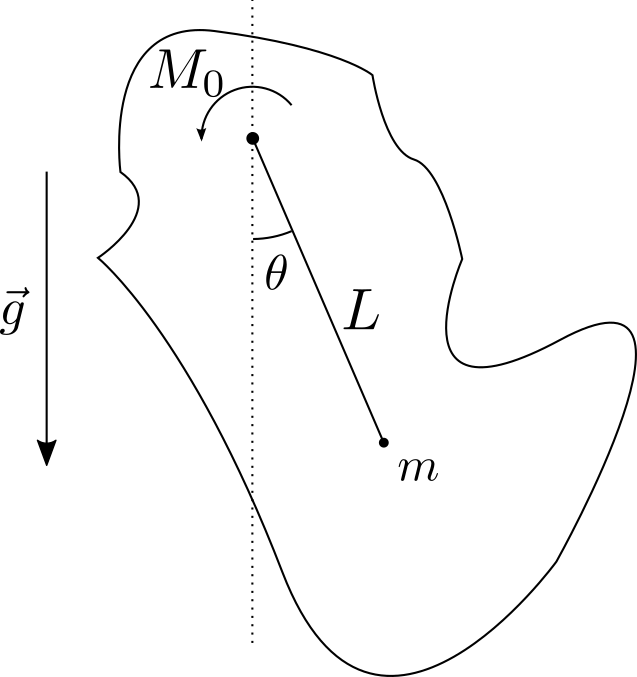
\includegraphics[scale=0.7]{pendulum.png}
\caption{Setup of a typical physical pendulum and notation used to describe it.}
\label{fig:setup}
\end{figure}

To describe a physical pendulum we use the rotational equivalent of Newton's II. law to write down a differential equation for the angular variable $\theta$;
%
\begin{align}
I \ddot{\theta} = -mgl \sin(\theta) - b \dot{\theta} + M_0 \sin(\tilde{\omega} t).
\end{align}

This equation, as usual, has the restorative torque due to gravity $-mgl\sin(\theta)$, where $m$ is the mass, $g$ the acceleration due to gravity, and $l$ is the distance between the pivot and the center of mass of the pendulum.

We have also included a damping term $-b \dot{\theta}$, which we know reigns in the infinities we get exactly at resonance, at least in the linear approximation of the problem.

The final term is the driving torque $M_0 \sin(\tilde{\omega} t)$, where $M_0$ is the driving amplitude and $\tilde{\omega}$ is the driving angular frequency.

To get a better grasp on how the values of the parameters influence the equation and eventual solution we perform a nondimensionalization. Defining the quantities
%
\begin{align}
&\omega_0^2 = \frac{mgl}{I},& &\gamma = \frac{b}{2I \omega_0},& &\psi_0 = \frac{M_0}{I \omega_0^2},&
\end{align}
%
and further redefining time as $\tau = \omega_0 t$ (while continuing to use dot notation to mean derivative with respect to $\tau$) and the driving frequency as $\omega = \tilde{\omega}/\omega_0$, we get the nondimensional form
%
\begin{align}
\ddot{\theta} + 2\gamma \dot{\theta} + \sin(\theta) = \psi_0 \sin(\omega \tau).
\end{align}\label{eq:diffeq}


\section{Methods}

\subsection{Theoretical description}

Firstly, we will extract as much information about the solutions as possible analytically. We can do an analysis for $\psi_0 \gg 1$ by comparing terms. We see that $\sin(\theta) \ll \psi_0 \sin(\omega \tau)$, which conveniently lets us neglect the non-linear term so that our equation becomes
%
\begin{align}
\ddot{\theta} + 2\gamma \dot{\theta} \sim \psi_0 \sin(\omega \tau) \quad (\psi_0 \gg 1).
\end{align}

This is a linear equation with the solution
%
\begin{align}
\theta &\sim - \frac{\psi_0}{\omega \sqrt{\omega^2 + 4\gamma^2}} \sin\left(\omega \tau + \arctan\left(\frac{2 \gamma}{\omega}\right)\right),
\end{align}
%
where the homogeneous part of the solution is subdominant for $\psi_0 \gg 1$. Thus, we get that the response $\rho(\omega)$ for large driving amplitudes is
%
\begin{align}
\rho(\omega) \sim \frac{\psi_0}{\omega \sqrt{\omega^2 + 4\gamma^2}} \quad (\psi_0 \gg 1).
\end{align}

In a similar fashion, we can look at the limiting case $\omega \rightarrow 0 $. For this we actually need to use a different nondimensionalization, where we have $x = \omega \tau$ and the equation is
%
\begin{align}
\omega^2 \theta'' + 2 \gamma \omega \theta' + \sin(\theta) = \psi_0 \sin(x)
\end{align}

In the limit of small $\omega$ we have the asymptotic relations
%
\begin{align}
\sin(\theta) &\sim \psi_0 \sin(\omega \tau) \\
\theta &\sim \arcsin(\psi_0 \sin(\omega \tau)) \quad (\omega \ll 1)
\end{align}
%
but we notice that for $\psi_0 > 1$ the derivatives of $\theta$ have infinite divergences; there our asymptotic analysis is not valid because we threw away the derivative terms under the assumption that they were finite and a small enough $\omega$ existed to make them negligible. So we get that in the regime $\psi_0 < 1$, the response is given by
%
\begin{align}
\rho(\omega) \sim \arcsin(\psi_0) \quad (\omega \ll 1,\, \psi_0 \leq 1)
\end{align}


Another way to approach a non-linear problem like this is through perturbation theory. Therefore, we insert a small parameter $\epsilon$ into equation \ref{eq:diffeq} that will help us linearize it
%
\begin{align}
\ddot{\theta} + 2\gamma \dot{\theta} + \sin(\epsilon \theta) = \psi_0 \sin(\omega \tau)
\end{align}
%
and we look for a solution of the form
%
\begin{align}
\theta(\tau) = \sum_{\alpha=0}^{\infty} \theta_{\alpha}(\tau) \, \epsilon^{\alpha}.
\end{align}

In the end, we will set $\epsilon = 1$ to get information about the solution of the original equation. (We will, in general, not get the full solution because of convergence issues for the infinite sums)

Using the Taylor expansion $\sin(x) = \sum_{n=0}^{\infty} \frac{(-1)^n}{(2n+1)!} x^{2n+1}$ for sine and writing the first few terms in powers of $\epsilon$, we get
%
\begin{align}
\sin(\epsilon \theta) &= \epsilon \left[\theta_0\right] + \epsilon^2 \left[\theta_1\right] + \epsilon^3 \left[\theta_2 - \frac{1}{6} \theta_0^3\right]\notag\\ &+ \epsilon^4 \left[\theta_3 - \frac{1}{2}\theta_1\theta_0^2\right] + \mathcal{O}(\epsilon^5),
\end{align}
%
giving us the equations
%
\begin{align}
\ddot{\theta_0} + 2\gamma \dot{\theta_0} &= \psi_0 \sin(\omega \tau) \label{eq:theta_0}\\
\ddot{\theta_1} + 2\gamma \dot{\theta_1} &= -\theta_0 \\
\ddot{\theta_2} + 2\gamma \dot{\theta_2} &= -\theta_1 \\
\ddot{\theta_3} + 2\gamma \dot{\theta_3} &= -\theta_2 + \frac{1}{6}\theta_0^3 \\
&...\notag
\end{align}

In general, the solutions for the different $\theta_{\alpha}$ will be some combination of a constant part, a polynomial of degree $\leq \alpha$ times a decaying exponential (the infinite sum of which conspires to form the decaying oscillation of the system without driving) and an oscillatory part due to the driving or some product thereof.

Equation \ref{eq:theta_0} is the same equation we solved previously, so we see the appearance of the factor $\zeta = \left(\sqrt{\omega^4 + 4 \gamma^2 \omega^2}\right)^{-1}$ again. Every consecutive $\theta_{\alpha}$ term will have at least one extra copy of $\zeta$, meaning that asymptotically, for large $\omega$ we again have the response amplitude being
%
\begin{align}
\rho(\omega) \sim \frac{\psi_0}{\sqrt{\omega^4 + 4 \gamma^2 \omega^2}} \sim \frac{\psi_0}{\omega^2} \quad \quad (\omega \gg 1),
\end{align}
%
but this time regardless of the size of the driving amplitude $\psi_0$.

The effect of the non-linear terms from the sine expansion is to include higher frequencies, which are integer multiples of $\omega$. This can be seen from the fact that powers of sine and cosine can always be written as combinations of sines and cosines with different frequencies.

\subsection{Numerical description}

Although the system we are describing is, in general, chaotic, we are only examining the steady state solution, which is independent of initial conditions. The reason for this is friction; it erases the system's knowledge of the initial conditions the closer we get to the steady state. Therefore, we won't have the usual problems that come with numerically solving a chaotic system.

The strategy we will use is to solve the differential equation in chunks of one period $2 \pi / \omega$ and compare the solution in consecutive chunks. We stop solving the equation when the solution is the same in the two chunks, up to some tolerance, or if it seems like the solution isn't converging to an oscillation.

The definition of amplitude is complicated slightly by the fact that multiple frequencies can be present in the steady state oscillation. But because the resonant response should, in the end, be a measure of how wildly the system is oscillating, we will choose the simplest possible definition of amplitude -- half of the difference between the maximum and minimum during a period.


\section{Results and Discussion}

We have made analytic predictions for the four limiting cases $\psi_0 \ll 1$, $\psi_0 \gg 1$, $\omega \ll 1$, and $\omega \gg 1$, so we will test them first.

\begin{figure}
\centering
\captionsetup{justification=centering}
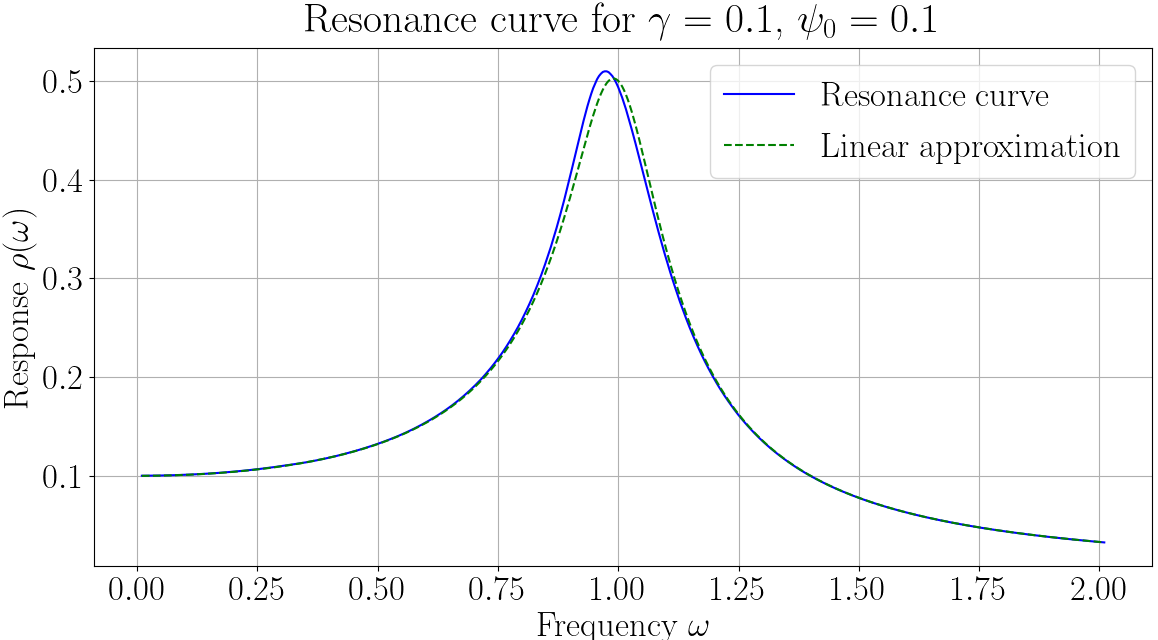
\includegraphics[scale=0.25]{small_amp.png}
\caption{Numerical (blue, solid) and theoretical (green, dashed) results for relatively small angles.}
\label{fig:small_amp}
\end{figure}

Looking at figure \ref{fig:small_amp}, we see that for small angles, using $\psi_0 = 0.1$, we get good agreement with the usual formula
%
\begin{align}
\rho(\omega) \sim \frac{\psi_0}{\sqrt{(\omega^2-1)^2 + (2\gamma\omega)^2}} \quad (\psi_0 \ll 1).
\end{align}

\begin{figure}[h]
\centering
\captionsetup{justification=centering}
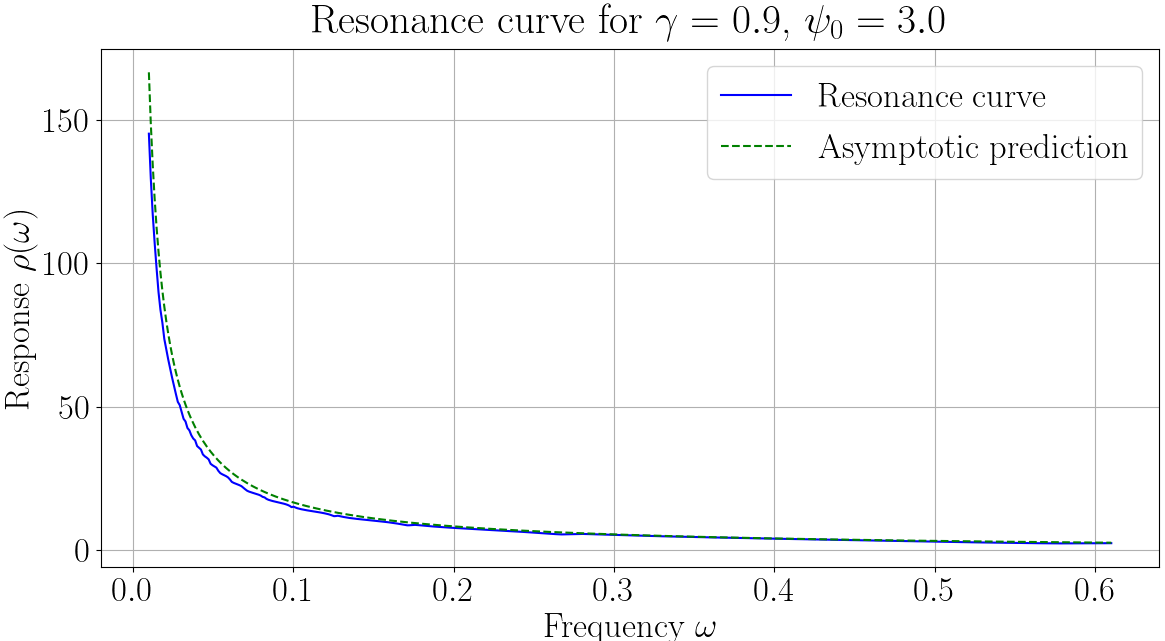
\includegraphics[scale=0.25]{large_amp.png}
\caption{Numerical (blue, solid) and theoretical (green, dashed) results for large driving amplitude.}
\label{fig:large_amp}
\end{figure}

Figure \ref{fig:large_amp} shows the same but for large amplitudes, in this case $\psi_0 = 3.0$. A damping factor of $\gamma = 0.9$ had to be taken for the solution to converge to an oscillation in less than $500\,000$ period chunks. We see that for all $\omega$ in the figure the agreement is pretty good, with it becoming gradually worse the smaller $\omega$ is.

\begin{figure}
\centering
\captionsetup{justification=centering}
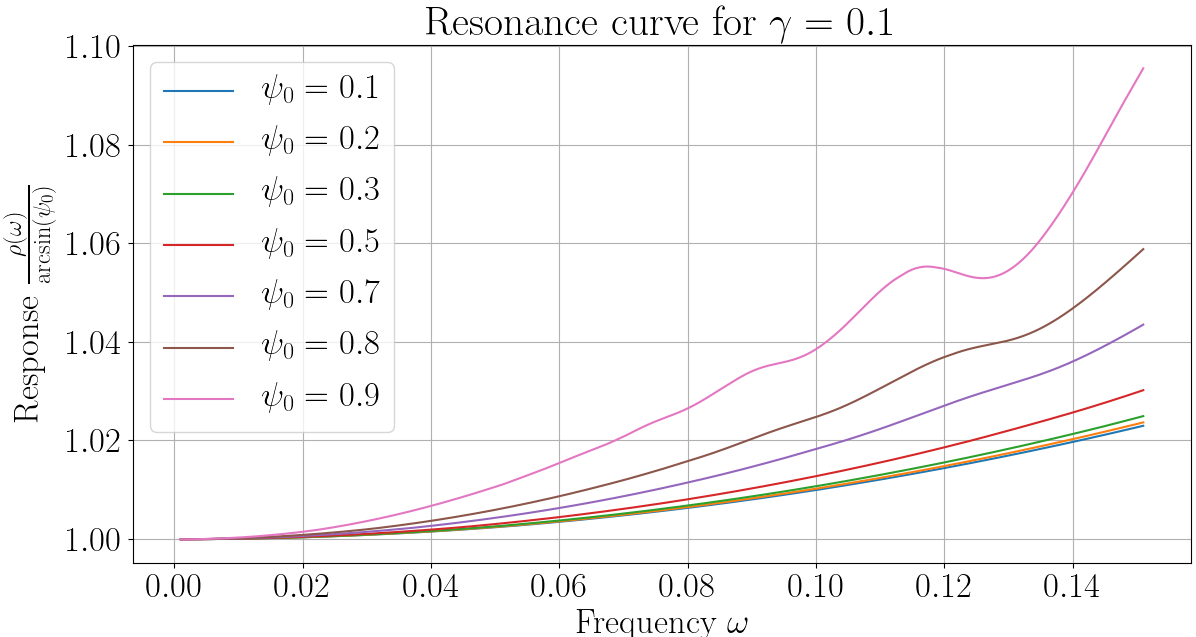
\includegraphics[scale=0.25]{small_freq.png}
\caption{The resonant response in the range of small frequencies scaled by $\arcsin(\psi_0)$ for a few different $\psi_0$.}
\label{fig:small_freq}
\end{figure}

With figure \ref{fig:small_freq} we test our prediction for small $\omega$. It shows the scaled resonant response $\frac{\rho(\omega)}{\arcsin(\psi_0)}$ in the small frequency range, for a couple of different $\psi_0$, which are necessarily smaller than $1$. We see that they all converge to $1$ as we expected from our analysis, but also that the convergence is slower the closer $\psi_0$ is to $1$.

While we were limited in analytically determining the behavior of $\rho(\omega)$ for small $\omega$ and $\psi_0 > 1$, numerically we can see that a transition happens at $\psi_0 = 1$. For values larger than that, $\rho(\omega)$ starts blowing up to infinity in the vicinity of $\omega = 0$. We already saw this singularity for large driving amplitudes, but now we've strengthened the condition for its appearance.

\begin{figure}[h]
\centering
\captionsetup{justification=centering}
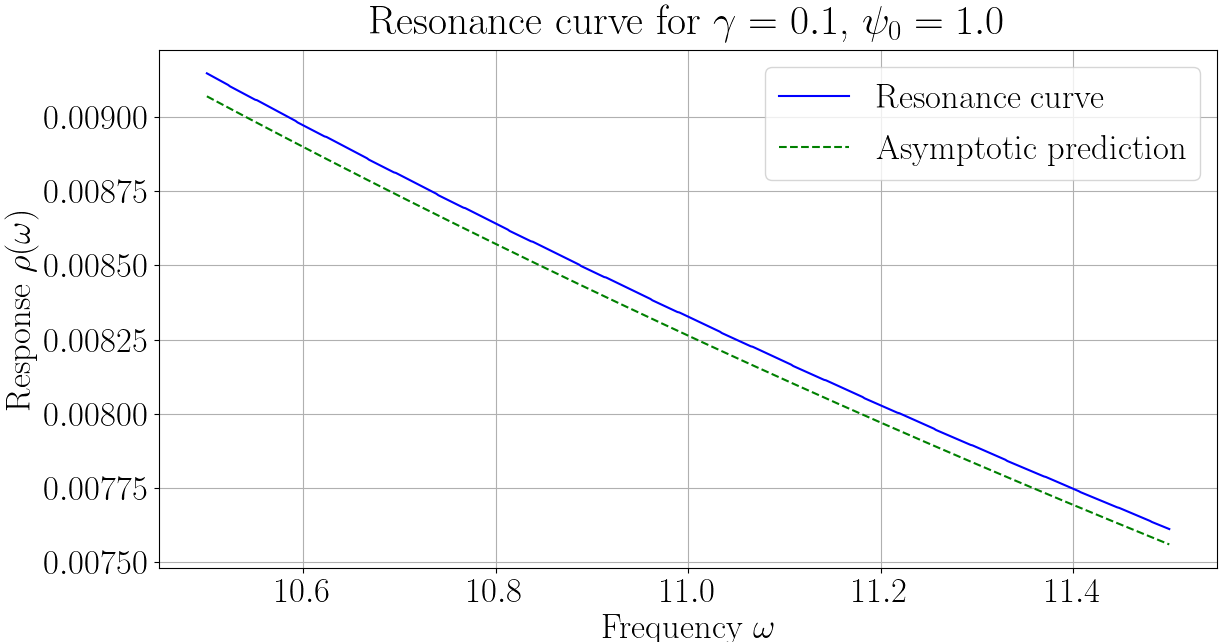
\includegraphics[scale=0.25]{large_freq.png}
\caption{Numerical (blue, solid) and theoretical (green, dashed) results for frequency.}
\label{fig:large_freq}
\end{figure}

In figure \ref{fig:large_freq} we can see the behavior for large frequencies, specifically $\omega \in [10.5, 11.5]$, for a driving amplitude of $\psi_0 = 1.0$ and damping $\gamma = 0.1$. We see that the asymptotic approximation for large $\omega$ does a pretty good job even for $\omega = \mathcal{O}(10)$. Knowing about the transition at $\psi_0 = 1.0$ we also double-check the result with small and large driving amplitudes, but the plots look nearly identical.

\begin{figure}
\centering
\captionsetup{justification=centering}
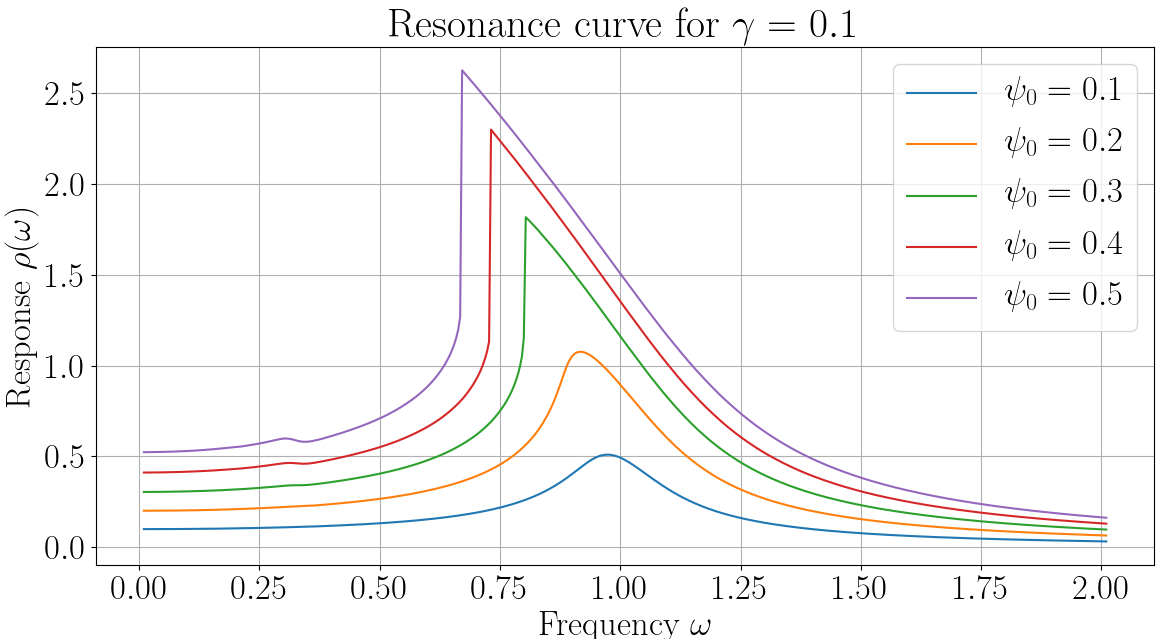
\includegraphics[scale=0.25]{medium_amp.png}
\caption{Resonance curves for different driving amplitudes and a damping factor of $\gamma=0.1$.}
\label{fig:medium_amp}
\end{figure}

Figure \ref{fig:medium_amp} shows the resonant response for a damping factor of $\gamma=0.1$ and different driving amplitudes, starting from the previous $\psi_0=0.1$ and going into the medium range. The first thing we notice is that the peak of the resonance curve gets shifted to lower frequencies and its left side becomes much steeper as we go to higher and higher driving amplitudes. Furthermore, we see a secondary peak start to appear at around $\omega \approx 0.31$. For larger amplitudes and smaller damping even more secondary peaks start to appear at lower frequencies.

\begin{figure}[h]
\centering
\captionsetup{justification=centering}
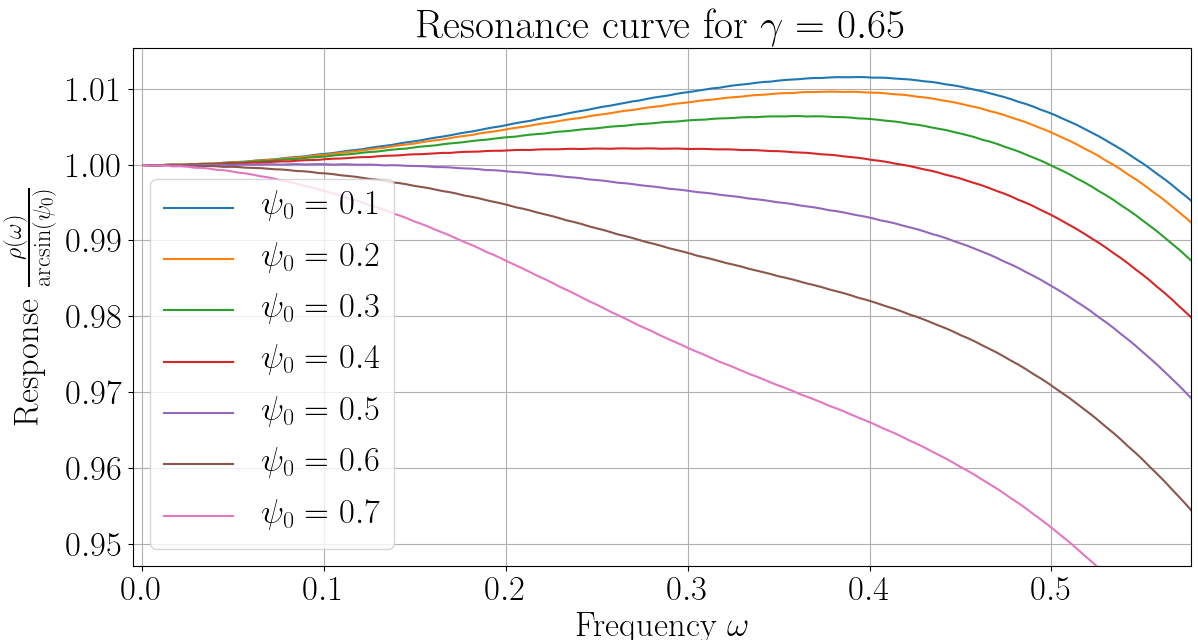
\includegraphics[scale=0.25]{trans_gamma.png}
\caption{Resonance curves for different driving amplitudes and a damping factor of $\gamma=0.65$.}
\label{fig:trans_gamma}
\end{figure}

For driving amplitudes $\psi_0 < 1$ the system displays the same critical damping behavior as the linearized version. Namely, the resonance curve doesn't have the characteristic local maximum for large damping. In the linear case that happens if $\gamma > \gamma_{\mathrm{crit.}} = 1/\sqrt{2} \approx 0.707$. That critical value, however, does not remain the same across different $\psi_0$; its value is largest in the small amplitude case and then it gradually decreases down to about $\gamma_{\mathrm{crit.}}(\psi_0 = 1.0) \approx 0.569$.

Figure \ref{fig:trans_gamma}, similarly to figure \ref{fig:small_freq}, is a plot of the scaled response amplitude $\frac{\rho(\omega)}{\arcsin(\psi_0)}$ given a damping factor of $\gamma = 0.65$, for a few different $\psi_0$. At this value of $\gamma$ some of the curves with higher driving amplitudes have already transitioned into the no local maximum regime, while the lower driving amplitude curves still have their local maxima.

For higher driving amplitudes and lower damping factors we get into convergence issues of two types. One is purely practical in that we have to cut off the numerical process at some point just to get feasible running times. The second type is that for some combination of $\gamma$, $\psi_0$, and $\omega$ we don't get a solution that can be considered periodic in any sense of the word. 

Figure \ref{fig:converg_issues} is an example of that; its driving amplitude of $\psi_0 = 0.7$ and slight damping $\gamma = 0.1$ conspire to form a couple of regions in the frequency range, around the peak, where the solution doesn't converge to an oscillation in the given number of steps, namely, $150$ per chunk with $3\,300$ chunks.


\begin{figure}[h]
\centering
\captionsetup{justification=centering}
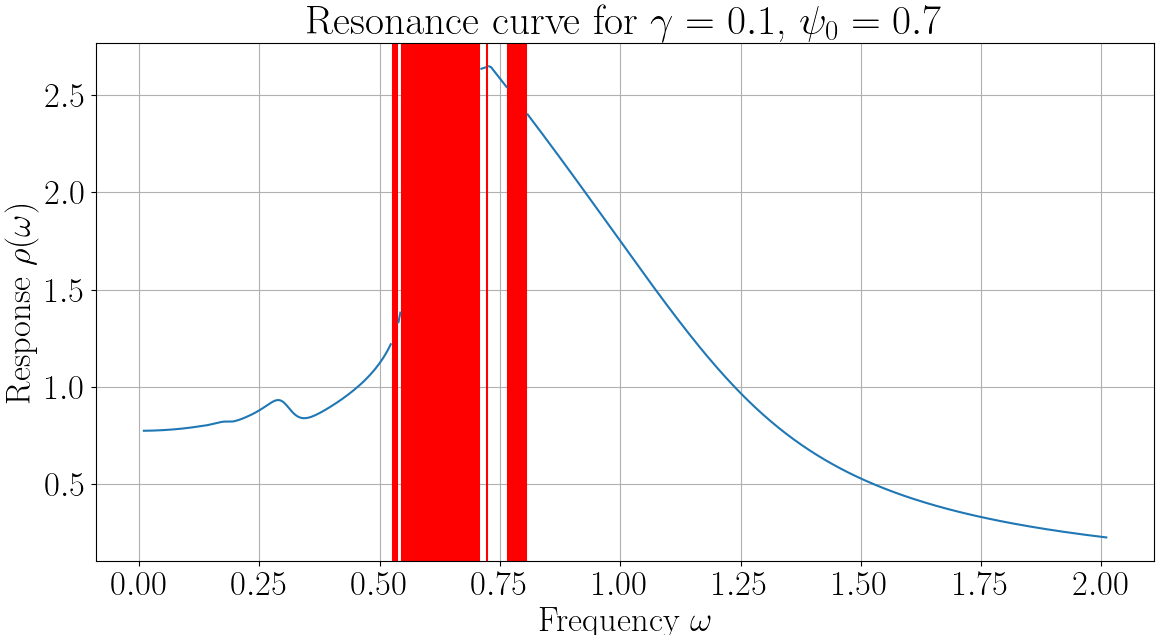
\includegraphics[scale=0.25]{converg_issues.png}
\caption{Resonance curve for $\psi_0 = 0.7$ and $\gamma = 0.1$. Region where solution didn't converge shown in red.}
\label{fig:converg_issues}
\end{figure}

\section{Notes}

The code used to simulate the differential equations can be found at \href{https://github.com/ackiivanov/nonlin-resonance}{github.com/ackiivanov/nonlin-resonance}

\end{document}